% Prompt-Injection Portfolio — Program Review (corrected native build)
% Engine: lualatex (latexmk -lualatex). Style: KOMA scrartcl, Roboto sans body.
% Supersedes the pandoc program-review-2026-06.md (deleted). Internal decision-support.
\documentclass[11pt,parskip=half-]{scrartcl}

\usepackage[letterpaper,margin=1in]{geometry}
\usepackage{fontspec}
\usepackage[sfdefault]{roboto}      % Roboto as default (sans) family
\usepackage{amsmath,amssymb}
\usepackage{microtype}
\usepackage{booktabs}
\usepackage{tabularx}
\usepackage{array}
\usepackage{enumitem}
\usepackage{xcolor}
\usepackage[most]{tcolorbox}
\usepackage{tikz}
\usetikzlibrary{positioning,arrows.meta,shapes.geometric,fit,backgrounds,calc}
\usepackage{xspace}
\usepackage[colorlinks=true,linkcolor=accent,urlcolor=accent,citecolor=accent]{hyperref}

% --- warm palette ------------------------------------------------------------
\definecolor{ink}{HTML}{2A2A2A}
\definecolor{accent}{HTML}{B5651D}      % warm ochre/terracotta
\definecolor{accentdk}{HTML}{8A4B12}
\definecolor{shown}{HTML}{2E7D5B}       % muted green (shown)
\definecolor{openred}{HTML}{B23A2E}     % muted red (open)
\definecolor{paper}{HTML}{FBF7F0}
\definecolor{soft}{HTML}{F1E9DC}
\definecolor{rule}{HTML}{D8CcB8}
\color{ink}

% --- KOMA section fonts ------------------------------------------------------
\setkomafont{title}{\bfseries\color{accentdk}}
\setkomafont{section}{\Large\bfseries\color{accentdk}}
\setkomafont{subsection}{\large\bfseries\color{accent}}
\setkomafont{subsubsection}{\normalsize\bfseries\color{ink}}
\addtokomafont{disposition}{\rmfamily}\addtokomafont{disposition}{\sffamily}

% --- helpers -----------------------------------------------------------------
\newcommand{\arr}{\ensuremath{\rightarrow}}
\newcommand{\lra}{\ensuremath{\leftrightarrow}}
\newcommand{\approxsym}{\ensuremath{\approx}}
\newcommand{\X}{\ensuremath{\times}}
\usepackage{seqsplit}
\newcommand{\code}[1]{\texttt{\small #1}}
\newcommand{\lpath}[1]{\texttt{\small\seqsplit{#1}}}   % breakable long file paths

% Key-finding (shown) callout
\newtcolorbox{shownbox}[1][What this means]{%
  colback=soft,colframe=shown,coltitle=white,
  fonttitle=\bfseries,title={#1},
  boxrule=0.8pt,arc=2pt,left=6pt,right=6pt,top=4pt,bottom=4pt,
  breakable}

% Open-question callout
\newtcolorbox{openbox}[1][Open]{%
  colback=openred!6,colframe=openred,coltitle=white,
  fonttitle=\bfseries,title={#1},
  boxrule=0.8pt,arc=2pt,left=6pt,right=6pt,top=4pt,bottom=4pt,
  breakable}

% Insight callout (educational)
\newtcolorbox{insightbox}[1][Insight]{%
  enhanced,colback=paper,colframe=accent,coltitle=accentdk,
  fonttitle=\bfseries,title={#1},
  boxrule=0.6pt,arc=2pt,left=6pt,right=6pt,top=4pt,bottom=4pt,
  borderline west={2.5pt}{0pt}{accent},
  breakable}

\newcolumntype{Y}{>{\raggedright\arraybackslash}X}

\setlist[itemize]{leftmargin=1.3em,itemsep=2pt,topsep=2pt}

% =============================================================================
\title{Prompt-Injection Portfolio --- Program Review}
\subtitle{\normalsize\mdseries\color{accent}What we've done {\(\times\)} what we can do --- a corrected review before the next line of work}
\date{2026-06-02 \quad\textbar\quad internal decision-support}
\author{}

\begin{document}
\maketitle
\thispagestyle{empty}

% =============================================================================
\section*{Executive summary}
\addcontentsline{toc}{section}{Executive summary}

The project set out to test whether prompt-injection \emph{detectors} hit an ``OOD wall'' --- they
work on data like their training set and fail on data unlike it. \textbf{Two within-corpus axes are now
answered, independently re-checked five times ($\Delta \le 10^{-4}$), for about \$2 of a \$250 budget}
--- and that is real, audited progress worth banking:

\begin{itemize}
  \item \textbf{Attack-type axis} (generalising to a \emph{kind} of attack never seen, inside BIPIA):
    the wall is \textbf{real for weak detectors but dissolves once you fine-tune} ---
    \emph{capacity-dependent}. A small fine-tune (LoRA) detects every held-out attack-type
    near-uniformly.
  \item \textbf{Carrier axis} (generalising to a new \emph{container} --- email vs.\ code vs.\ table,
    inside BIPIA): the wall is \textbf{only partly removed by fine-tuning} --- it shrinks
    ${\sim}60\%$ but leaves a \textbf{stubborn residual gap on table-formatted inputs} ---
    \emph{capacity-attenuated}.
\end{itemize}

\textbf{But both axes live inside a single corpus (BIPIA).} The prototype's original wall was a
different and harder thing: \emph{direct\arr indirect transfer across different datasets} ---
``cross-family''. That wall is real at the un-confounded \emph{frozen} probe (it sits at chance), and it
was \textbf{never re-run under fair tuning}. So the sharpest question is the \emph{symmetric} one: the
portfolio showed that fair-tuned capacity \emph{dissolves} the attack-type wall --- does fair-tuned
capacity \emph{climb} the cross-family wall the same way? That is \textbf{untested}. Naming this honestly
is the spine of this review.

\begin{openbox}[The one-sentence state of play]
We answered the two \emph{within-BIPIA} axes (attack-type dissolves; carrier attenuates). Whether
fair-tuned capacity climbs the prototype's \emph{cross-family} wall is the single sharpest \textbf{OPEN}
question --- and the cheap experiment that would settle it is the recommended next step.
\end{openbox}

\subsection*{The three walls (one frame)}
The two repositories never measured the \emph{same} wall; their headlines only \emph{appear} to collide.
Separating the axes dissolves the apparent contradiction:

\begin{center}\small
\begin{tabularx}{\linewidth}{@{}l l Y l@{}}
\toprule
\textbf{Axis} & \textbf{Scope} & \textbf{What's shown} & \textbf{Status} \\
\midrule
Attack-type & within BIPIA (\emph{kind} of attack) &
  real at tfidf/frozen; dissolves at LoRA ($T$: $+0.135 \arr +0.082 \arr -0.003$) &
  \textcolor{shown}{capacity-dependent} \\[4pt]
Carrier & within BIPIA (\emph{container}) &
  frozen $G\,{+}0.167 \arr$ lora $+0.067$; residual table $+0.205$ &
  \textcolor{shown}{capacity-attenuated} (n=3) \\[4pt]
Cross-family & across datasets (direct\arr indirect) &
  frozen probe at chance (AUPRC $0.364 \le 0.374$ floor); fair-tuned capacity never re-run &
  \textcolor{openred}{\textbf{OPEN}} --- critical next test \\
\bottomrule
\end{tabularx}
\end{center}

\subsection*{Milestones \& the decision}
\textbf{M0} (planning + analysis) and \textbf{M1} (the attack-type study) are done and ratified; the
\textbf{carrier pre-flight} is done; \textbf{M2--M7 have not started.} So the two \emph{within-BIPIA}
science questions are settled and audited; the harder cross-family question is open; the
\emph{build-out} (remaining lanes, the book) is almost entirely ahead --- and mostly a \textbf{choice},
not a necessity.

\textbf{The decision this document supports:} \emph{consolidate} (write up + publish what's proven) vs.\
\emph{advance} (run more lanes) --- with one new, cheap, high-stakes option now sitting at the front:
the \textbf{cross-family fair-tuning re-run}. Doing \emph{everything} still fits inside \$250.

% =============================================================================
\section{What we've done}

\subsection{Results \& verdicts (all verified)}

\begin{center}\small
\begin{tabularx}{\linewidth}{@{}l Y Y@{}}
\toprule
\textbf{Study} & \textbf{Verdict} & \textbf{Key numbers} \\
\midrule
\textbf{M1 attack-type-LODO} (\S6.5 OOD-wall prediction) &
  \textbf{FALSIFIED at the LoRA ceiling --- capacity-dependent} &
  tfidf $T={+}0.135$ (p .014) / frozen ${+}0.082$ (p .014) \textbf{SURVIVE}; \textbf{lora $-0.003$
  (p .90) FALSIFIED}; LoRA per-type AUPRC \textbf{0.956--0.984} \\[5pt]
\textbf{Carrier-LODO} (M2 pre-flight) &
  \textbf{SMALL-THROUGHOUT --- capacity-attenuated, residual at table} &
  frozen $G={+}0.167 \arr$ \textbf{lora ${+}0.067$} (CI-low ${+}0.064$; ${\sim}60\%$ attenuation);
  per-carrier at lora: email $-0.012$ / code ${+}0.007$ / \textbf{table ${+}0.205$} \\[5pt]
\textbf{EDA geometry} (pre-modeling) &
  carrier dominates; attack-type embedding-invisible (on \emph{frozen MiniLM}) &
  silhouette by-carrier \textbf{0.197} vs by-attack-type $-0.023$; KMeans\arr carrier ARI \textbf{0.98}
  vs $-0.001$ \\[5pt]
\textbf{Off-the-shelf detectors} (V10) &
  consistent with scope-blindness, not undetectable data &
  ProtectAI \textbf{AUROC 0.44} (worse than chance); Prompt-Guard-86M 0.86 attack / 0.04 benign
  (AUROC 0.97) \\[5pt]
\textbf{Independent audit} (5 verifiers) &
  \textbf{5/5 reproduce, $\Delta \le 10^{-4}$, no mismatch} &
  every headline statistic re-derived independently \\
\bottomrule
\end{tabularx}
\end{center}

\subsection{The finding, scoped to its axis}

\begin{quote}
\textbf{On the attack-type axis, within BIPIA indirect injection}, the OOD ``wall'' is a property of the
\textbf{representation, not the task}: real for lexical / frozen-embedding detectors, and surmountable by
a small amount of end-to-end capacity, which detects every held-out attack-type near-uniformly (test
AUPRC \textbf{0.956--0.984}). \textbf{On the carrier axis}, it is only \emph{partially}
capacity-resistant --- a residual wall at tabular contexts ($+0.205$, n=3, provisional).
\textbf{Across families} (the prototype's direct\arr indirect, cross-dataset wall), whether fair-tuned
capacity climbs it is \textbf{open}.
\end{quote}

\begin{insightbox}[Two caveats on ``dissolved'']
\textbf{(a) Ceiling-compression (a bound, not a refutation).} At the LoRA rung the per-type AUPRCs all
sit near the upper bound (0.956--0.984, well above the ${\sim}0.926$ no-skill floor). The statistic
$T$ is a top-$k$ minus bottom-$k$ \emph{difference} of those levels, so with everything pinned near
ceiling the contrast is mechanically compressed toward zero: $T\arr 0$ reflects \emph{uniform
near-ceiling detection} as much as a ``dissolved'' gap. This \emph{bounds} how triumphantly we can read
``dissolved'' --- it does \emph{not} undermine the FALSIFIED verdict, whose rule, tails, $k$, and
estimator were fixed before any LoRA datum and write-gated.\\[2pt]
\textbf{(b) Within-corpus.} The held-out attack-type shares carrier, corpus, and generating process
with the training types --- this is \emph{within-corpus} generalization, the expected easy case, not
the demanding \emph{cross-family} test.
\end{insightbox}

\subsection{Consistency with the pre-modeling EDA}

The EDA was computed on the \textbf{frozen MiniLM} embedding (\emph{not} the ModernBERT detector
backbone), so it could only ever describe how \emph{frozen / lexical} detectors behave --- and the
modeling confirmed it exactly there:

\begin{itemize}
  \item The per-type prediction \textbf{SURVIVES at tfidf and frozen} (the representation it was derived
    from) and dissolves only at LoRA --- the capacity axis the EDA was blind to by construction.
  \item The EDA's single biggest call was the \textbf{bullseye}: it named the \emph{carrier} (not the
    attack-type) as the real wall \emph{before any model ran}; the carrier-LODO then found exactly that
    residual carrier wall.
  \item The off-the-shelf reading (V10) held: direct-trained probes are \emph{consistent with}
    scope-blindness to indirect injection (ProtectAI AUROC 0.44), while the indirect-capable probe fires
    (PG1 AUROC 0.97). (This is an \emph{interpretation} of a below-chance score; the portfolio's own
    prescription --- demonstrate it with per-row score distributions --- is not yet run, hence the
    softened wording.)
\end{itemize}

\subsubsection{Two framing corrections folded into this review}

\begin{enumerate}[leftmargin=1.4em]
  \item \textbf{S2 vs.\ capacity-dependence (fixed earlier this session).} An over-claim conflated the
    pre-registered S2 caveat (\emph{prediction-encoder choice} MiniLM \arr frozen ModernBERT --- the
    ranking \emph{transfers}, verified at the frozen rung) with the broader, not-pre-committed
    \emph{capacity} dissolution at LoRA. The two are now separated wherever they travel.
  \item \textbf{Cross-family scope (this review).} An independent second-opinion audit found the review
    layer generalized past the within-BIPIA axes (``answered on two axes''; ``property of the
    representation, not the task''). The boundary between what was \emph{shown} (within-BIPIA
    attack-type + carrier) and what was \emph{inherited / open} (the prototype's cross-family wall) is
    now drawn explicitly --- this whole document is the corrected version.
\end{enumerate}

\subsection{Fine-tuning status}
\begin{itemize}
  \item \textbf{LoRA --- done.} This \emph{is} the promising result; it dissolved the attack-type wall.
  \item \textbf{\code{full\_ft} (full fine-tune) --- deliberately not run.} Its trigger-gate resolved
    \emph{does-not-fire}. The \emph{expectation} is that more capacity than LoRA can only dissolve the
    attack-type wall further --- but note this is a \textbf{conjecture}: full-FT OOD was never measured
    (the prototype's attempt crashed; ADR-052/ADR-075), so it is an expectation, not a result.
  \item \textbf{Lane 2 (carrier-axis LoRA) --- the genuine next within-BIPIA fine-tune}
    (\S\ref{sec:paths}\,(3)); upstream-blocked.
  \item \textbf{Cross-family fair-tuned re-run --- the genuine \emph{open} fine-tune}
    (\S\ref{sec:paths}, critical \#1); unblocked.
\end{itemize}

\subsection{Budget \& milestones}
\begin{itemize}
  \item \textbf{M0} ratified; \textbf{v0.1.0 staged + held} for account creation (the public release).
  \item \textbf{M1} done + pushed; \textbf{carrier-LODO} done. \textbf{M2--M7 not started.}
  \item \textbf{Spend ${\approx}$ \$2 of the \$250 base budget.} The \$100 contingency reserve is
    untouched.
\end{itemize}

\subsection{This session's record-work (drafted, ratification-gated)}
A second-opinion audit produced a punch-list of framing/record fixes (A1--A8), drafted as
ratification-ready patches in \code{docs/planning/record-fixes-A1-A8.DRAFT.md} --- \emph{applied to no
canonical file} until ratified. They scope each shown result to its axis, mark cross-family OPEN, fix
two stale/record lines, and correct one prose over-round (per-type LoRA AUPRC \code{0.98--0.999}
\arr\ \code{0.956--0.984}, to match the artifact). The \textbf{ADR-055 carrier amendment} (downgrading
the spine's ``standing wall'' to ``partially capacity-resistant, provisional'') remains drafted and held;
its substance is in \textbf{Appendix~\ref{app:adr}}. Nothing is committed (commits are user-led).

% =============================================================================
\section{What we can do (the forward paths)}\label{sec:paths}

\subsection*{(\(\star\)) Critical \#1 --- Cross-family fair-tuning re-run \quad{\small ${\sim}$\$1--2, 2--3 days, unblocked}}

The audit's sharpest finding: the portfolio proved fair-tuned capacity \emph{dissolves the attack-type
wall}; the symmetric question --- does fair-tuned capacity \emph{climb the cross-family wall}? --- has no
clean answer, because the only cross-family fine-tune that exists is the prototype's confounded run.
Re-run it \emph{cleanly}: replicate the prototype's pooled-OOD slate (train
deepset/Gandalf/Mosscap/HackAPrompt \arr\ test BIPIA/InjecAgent/JBB/XSTest/NotInject) under the
portfolio's \emph{fair per-rung tuning} (ADR-052). The prototype already holds the configs + data slate.

\begin{openbox}[Why this is high-stakes, not cosmetic]
\textbf{Capacity climbs cross-family} \arr\ unifies both repositories; ``capacity-dependent''
generalizes; strongest possible story. \quad \textbf{Capacity fails cross-family} \arr\ the headline is
true only on the easy within-corpus axis; \emph{cross-family is the real standing wall} and the central
claim narrows sharply. Either outcome is publishable and pre-registered.
\end{openbox}

A lightweight pre-registration skeleton is drafted at
\lpath{experiments/cross-family-transfer/criteria.DRAFT.md} (both statistics named: prototype-comparable
pooled-OOD AUPRC-vs-floor + AUROC anchor, \emph{and} a cross-rung transfer-gap as the decision
statistic). The paid GPU run itself stays a separate present-first go.

\subsection*{(1) Consolidate --- write up and ship what's already proven \quad{\small \$0}}
Turn the finished result into finished outputs --- \emph{no new experiments}:
\begin{enumerate}[leftmargin=1.4em]
  \item Apply the held \textbf{ADR-055 amendment} (Appendix~\ref{app:adr}) so the record stops calling
    the carrier wall a ``standing wall.''
  \item Write the two book chapters whose results are ready --- the OOD-wall story (Ch~7) and the
    baseline (Ch~8). \emph{(Their outlines exist; the prose is unwritten.)}
  \item Close \textbf{v0.1.0} (tag + public release).
\end{enumerate}
\textbf{Value:} makes the audited result citable and the milestone public; resolves the open
record-vs-data gap. Highest credibility-per-dollar, lowest risk. \textbf{Needs:} a ratification and a
public release (your calls).

\subsection*{(2) Cheap-advance --- a small experiment while the big one is stuck \quad{\small ${\sim}$\$1 each, 2--3 days}}
\begin{itemize}
  \item \textbf{Lane 3 (spotlighting):} does \emph{marking} untrusted text (delimiters, or
    base64-encoding) --- known to make the LLM itself safer --- also make our \textbf{detectors} better?
    Inference-only; \textbf{feeds Lane 4}.
  \item \textbf{Lane 1b (character-injection):} do invisible characters / look-alike letters fool our
    detectors? (A 2025 paper fools \emph{older} detectors ${\sim}100\%$ of the time.) Includes a
    utility-aware robustness matrix.
\end{itemize}
\textbf{Value:} real findings (defence + robustness \emph{breadth}) with nothing blocking them --- but
these are side-quests, not the core carrier or cross-family story.

\subsection*{(3) Lane 2 --- can we TRAIN past the carrier wall? \quad{\small \$156--230, 4--5 weeks}}
The richest within-BIPIA next step. We found a stubborn gap on \textbf{table} inputs; Lane 2 asks whether
generating a big, carrier-diverse synthetic training set and retraining \textbf{closes} it.
\begin{itemize}
  \item \textbf{Currently blocked.} The tool that generates the synthetic data has a bug that could
    \emph{silently corrupt} the training set (research\_toolkit \#22 --- \S\ref{sec:blockers}). Options:
    fix it upstream first (small, drafted), use an existing corpus (cheaper, needs an agreement-quality
    check), or fall back to BIPIA-only data (unblocked now, but a narrower experiment).
  \item \textbf{The gateway.} Its training data is also what Lanes 4 and 5 need --- so little downstream
    runs without it.
  \item Even a \emph{null} result is publishable: the outcomes (data-bound / structural / worsened) were
    committed in advance.
\end{itemize}

\subsection*{(4) Carrier-settle --- make the carrier finding rock-solid \quad{\small \$0--2, 2--3 days once licensed}}
Our carrier result rests on \textbf{3} container types; \textbf{2 more} (qa, abstract) sit behind a
dataset license we don't have. Get the license, add them, re-run \arr\ a \emph{settled, 5-point} finding
instead of \emph{directional, 3-point.} Cheap and quick \textbf{once licensed}, but the license is
external and may not come. \textbf{Optional polish} --- the current finding is already honestly flagged
\emph{provisional}, with a scheduled re-test trigger.

\subsection{How they fit together}

\begin{center}
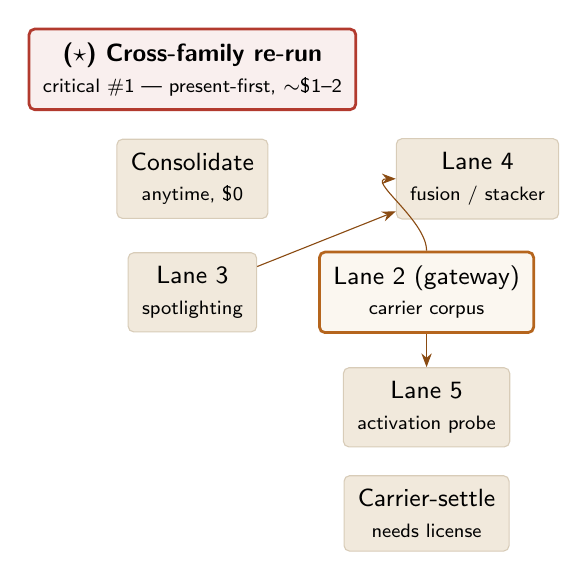
\begin{tikzpicture}[
  font=\sffamily\small,
  box/.style={rounded corners=2pt,draw=rule,fill=soft,inner sep=5pt,align=center,minimum height=2.2em},
  crit/.style={rounded corners=2pt,draw=openred,line width=1pt,fill=openred!8,inner sep=5pt,align=center},
  gate/.style={rounded corners=2pt,draw=accent,line width=1pt,fill=paper,inner sep=5pt,align=center},
  >={Stealth[length=5pt]},edge/.style={->,draw=accentdk}
]
\node[crit] (cf) {\textbf{($\star$) Cross-family re-run}\\\scriptsize critical \#1 --- present-first, ${\sim}$\$1--2};
\node[box,below=10pt of cf] (cons) {Consolidate\\\scriptsize anytime, \$0};
\node[box,below=12pt of cons] (l3) {Lane 3\\\scriptsize spotlighting};
\node[gate,right=22pt of l3] (l2) {Lane 2 (gateway)\\\scriptsize carrier corpus};
\node[box,right=46pt of cons] (l4) {Lane 4\\\scriptsize fusion / stacker};
\node[box,below=12pt of l2] (l5) {Lane 5\\\scriptsize activation probe};
\node[box,below=10pt of l5] (csettle) {Carrier-settle\\\scriptsize needs license};

\draw[edge] (l3) -- (l4);
\draw[edge] (l2.north) to[out=90,in=180] (l4.west);
\draw[edge] (l2) -- (l5);
\end{tikzpicture}
\end{center}

\begin{itemize}
  \item \textbf{Cross-family re-run is the gate to the headline's reach} --- it decides whether
    ``capacity-dependent'' is a within-corpus result or a general one.
  \item \textbf{Lane 2 is the gate to the program's back half} (Lanes 4 and 5 depend on its corpus).
  \item \textbf{Runnable now, no blocker:} Cross-family re-run, Consolidate, Lane 3, Lane 1b.
  \item \textbf{A sensible order:} Cross-family re-run (settle the reach) + Consolidate (bank it) \arr\
    Lane 3 (cheap, feeds Lane 4) \emph{while} pushing to unblock Lane 2 \arr\ Lane 2 \arr\ Lanes 4/5
    \arr\ carrier-settle if the license appears.
\end{itemize}

\subsubsection{Per-path summary}
\begin{center}\small
\begin{tabularx}{\linewidth}{@{}l l l Y Y@{}}
\toprule
\textbf{Path} & \textbf{Cost} & \textbf{Time} & \textbf{Blocker / gate} & \textbf{Adds} \\
\midrule
\textbf{($\star$) Cross-family re-run} & \$1--2 & 2--3 d & none (present-first) & does capacity climb the prototype's real wall \\
(1) Consolidate & \$0 & days & your ratify + accounts & publishable, citable result \\
(2) Lane 3 & \$0--1 & 2--3 d & none & does marking help detectors \\
(2) Lane 1b & \$1--3 & 2--3 d & none & char-injection robustness matrix \\
(3) Lane 2 & \$156--230 & 4--5 wk & \textbf{upstream \#22/\#23} (or fallback) & can training close the table wall \\
(4) Carrier-settle & \$0--2 & 2--3 d & \textbf{dataset license} & promotes provisional \arr\ settled \\
(5) Lane 4 & \$5--30 & 2--3 wk & needs prior-lane scores & multi-detector fusion + frontier \\
(6) Lane 5 & \$10--20 & 2--3 d & $d' > 0.5$ gate; needs Lane-2 corpus & signal in intermediate activations \\
(def) \code{full\_ft} & \$2--6 & ${\sim}$1 d & trigger says \emph{don't} & reviewer-proofing only \\
\bottomrule
\end{tabularx}
\end{center}

% =============================================================================
\section{Glossary (curated, hybrid)}
Each entry: an accurate definition, then a plain-language gloss. (The repo's full \code{docs/glossary.md}
has the complete set; this is the subset needed to read this review.)

\newcommand{\gloss}[1]{\textbf{#1}}
\begin{description}[leftmargin=0pt,style=unboxed,itemsep=3pt]
\item[] \gloss{Three walls / axes.} The OOD ``wall'' is not one thing: the \emph{attack-type} axis and
  the \emph{carrier} axis live within BIPIA; the \emph{cross-family} axis is across datasets
  (direct\arr indirect). \emph{In plain terms:} a detector can be surprised by \emph{what} the attack
  does, \emph{where} it hides, or \emph{which dataset} it comes from --- three different surprises.

\item[] \gloss{OOD (out-of-distribution).} Test data from a slice not seen in training. \emph{Plainly:}
  the detector is asked about something unlike anything it learned from.

\item[] \gloss{LODO (leave-one-domain-out).} Train on every domain but one, test on the held-out one,
  rotate; the domain is the attack-type (M1) or the carrier (carrier-LODO). \emph{Plainly:} hide one
  category during training and check the detector still handles it.

\item[] \gloss{Attack-type axis / Carrier axis.} The \emph{kind} of attack (14 BIPIA task-types) vs.\ the
  \emph{container} it rides in (email / code / table / qa / abstract). \emph{Plainly:} \emph{what} the
  attack does vs.\ \emph{where} it's hidden.

\item[] \gloss{Cross-family axis.} Across whole datasets: train on direct-injection corpora, test on
  indirect/mixed ones. The prototype's original wall. \emph{Plainly:} the hardest surprise --- a
  completely different source of attacks.

\item[] \gloss{Capacity ladder --- tfidf / frozen / LoRA / full\_ft.} Four detectors of increasing
  power: word-counts \arr\ a frozen language model's embeddings \arr\ a small fine-tune \arr\ a full
  fine-tune. \emph{Plainly:} dumbest to smartest; climbing it shows whether the wall is about the
  \emph{model} or the \emph{task}.

\item[] \gloss{capacity-dependent / -attenuated / residual wall.} A gap that \emph{vanishes} with model
  power / \emph{shrinks but persists} / \emph{the stubborn part left at the top}. \emph{Plainly:} does a
  bigger model erase the wall, only lower it, or leave a hard core?

\item[] \gloss{AUPRC vs AUROC.} Two accuracy scores. AUPRC is inflated when positives are common (BIPIA
  carriers are 83--94\% positive, so chance AUPRC ${\approx}0.92$); AUROC is balance-robust (0.5 =
  chance, below 0.5 = worse than chance). \emph{Plainly:} AUPRC can flatter a useless detector here;
  AUROC tells the truth --- which is why ProtectAI's 0.44 exposes it as scope-blind.

\item[] \gloss{transfer-gap (T) / ROC-gap (G).} The test statistics for two axes --- how much detection
  drops on a held-out attack-type ($T$) or carrier ($G$). \emph{Plainly:} the measured height of the
  wall.

\item[] \gloss{SURVIVES / FALSIFIED / SMALL-THROUGHOUT.} The three pre-committed verdicts: the wall is
  real and resists fine-tuning / is statistically gone / is real but only partly resists. \emph{Plainly:}
  the wall stands, falls, or partly-stands --- decided by a rule fixed in advance.

\item[] \gloss{pre-registration / write-gate.} Writing the hypothesis and decision rule \emph{before}
  seeing data; the write-gate forbids computing the verdict until all experiments have run.
  \emph{Plainly:} call your shot first, and don't peek.

\item[] \gloss{permutation p / bootstrap CI.} ``Could this be a fluke?'' (reshuffle labels) and ``is it
  reliably above zero?'' (resample). \emph{Plainly:} two sanity checks a result must pass.

\item[] \gloss{payload-clustered bootstrap.} Resampling correlated groups (the ${\sim}5$ strings per
  type) rather than rows. \emph{Plainly:} don't pretend correlated examples are independent.

\item[] \gloss{silhouette / ARI.} Clustering-geometry scores; by-carrier 0.197 vs by-attack-type
  $-0.023$ means the data clump by container, not attack-type --- \textbf{on the frozen MiniLM
  embedding} (not the ModernBERT detector backbone). \emph{Plainly:} that embedding ``sees'' the carrier
  and is blind to the attack-type.

\item[] \gloss{embedding-invisible.} A signal absent from the frozen embedding yet learnable end-to-end.
  \emph{Plainly:} the clue isn't in the model's frozen snapshot, but it can learn to see it if trained.

\item[] \gloss{$\kappa$ (Cohen's kappa).} Chance-corrected annotator agreement; Lane 2 needs
  $\kappa \ge 0.5$ before trusting synthetic data. \gloss{$d'$ (d-prime).} How far apart two
  distributions are; Lane 5's go/no-go gate ($>0.5$). \gloss{PAD / MMD.} Two measures of how different
  the test set is from training.

\item[] \gloss{S2 (encoder-transfer caveat).} A pre-registered note that using one embedding model to
  \emph{predict} another's behaviour might not transfer (it did, at the frozen rung) --- distinct from
  the separate finding that \emph{fine-tuning} erases the attack-type wall.

\item[] \gloss{trigger-gate (\S16) / Tier A\,$\cdot$\,B\,$\cdot$\,C.} An ``if X happens, then do Y''
  promise written in advance / a budget ladder (free-local / cheap-paid / expensive-gated).
  \emph{Plainly:} deferring isn't dropping; expensive add-ons run only if cheaper results justify them.

\item[] \gloss{spotlighting / character-injection (ASR) / activation probe.} Marking untrusted text /
  evasion via weird characters (attack success rate) / reading internal activations to spot task-drift
  --- Lanes 3, 1b, 5.

\item[] \gloss{BIPIA / ProtectAI / Prompt-Guard.} The benchmark (indirect injection across carriers
  $\times$ attack-types) / off-the-shelf detectors (ProtectAI + PG2 are direct-trained and scope-blind;
  PG1 is indirect-capable and fires).
\end{description}

% =============================================================================
\section{Upstream blockers: research\_toolkit \#22 / \#23}\label{sec:blockers}
Both are OPEN and gate Lane 2's \emph{primary} data path (\code{/dataset-synthesize}, the tool that makes
the synthetic training corpus).

\paragraph{\#22 (P1 --- behavioral readiness).} The skill shipped without the toolkit's normal
post-ship ``dogfood'' check. Three confirmed problems (code fixes tracked in sibling issue \#21):
\begin{enumerate}[leftmargin=1.4em]
  \item \textbf{Silent-failure (the corpus-corruption risk):} the text-extraction function returns an
    empty string when a model response has no text block (a refusal, or a tool-only/thinking-only stop),
    with no warning --- and that empty string gets written straight into the training corpus. The fix
    (raise instead of silently returning empty) is ${\sim}10$ lines and drafted.
  \item \textbf{Fail-late:} the API-key check lives only in the CLI entry point, so a programmatic caller
    gets a deep SDK error instead of a friendly message.
  \item \textbf{No burn-in:} the skill was never exercised once against a real recipe and logged.
\end{enumerate}

\paragraph{\#23 (P2 --- installability).} The skill exists but isn't wired into the toolkit's install
lists, so a fresh agent following the README \textbf{cannot invoke it}. Fix: generate the install lists
from the skill files (one source of truth).

\paragraph{Net for Lane 2.} The primary path needs \#22 (especially the silent-failure fix) and \#23
resolved upstream --- both research\_toolkit-side and user-pushed. Until then, Lane 2 either waits or
uses the BIPIA-only fallback (narrower).

% =============================================================================
\appendix
\section{The held ADR-055 carrier amendment (draft)}\label{app:adr}
This formalizes the carrier-LODO verdict into the spine decision record. \textbf{Drafted, not yet
applied} --- included here so the pending decision can be reviewed alongside the rest. Full draft at
\code{docs/planning/adr-055-carrier-amendment.DRAFT.md}.

\textbf{What changes.} ADR-055 currently calls the carrier axis the \textbf{``standing wall.''} The
carrier-LODO verdict (SMALL-THROUGHOUT) shows that's too strong; the amendment rewords it to
\textbf{``partially capacity-resistant (provisional, n=3 carriers) --- capacity-attenuated, with a
residual wall at the table carrier,''} records the result in a dated ``Carrier-LODO resolution''
section, and registers a \S16 re-test gate (re-run at n=5 when the qa/abstract license unlocks).

\textbf{The recorded resolution (verbatim core):}
\begin{quote}\small
\textbf{Verdict: SMALL-THROUGHOUT.} Cross-rung gap $G$ = mean over held-out carriers of (val ROC-AUC
$-$ test ROC-AUC): tfidf $-0.156$ / frozen $+0.167$ (CI-low $+0.163$) / \textbf{lora $+0.067$ (CI-low
$+0.064$)}; per-carrier at lora email $-0.012$ / code $+0.007$ / \textbf{table $+0.205$}. Decision rule
(pre-registered): SURVIVES iff $G(\text{lora}) > 0$ \textbf{and} CI-low $> 0$ \textbf{and}
$G(\text{lora}) \ge \tfrac{1}{2}\,G(\text{frozen})$; FALSIFIED iff CI-low $\le 0$; else
SMALL-THROUGHOUT. Here CI-low $+0.064 > 0$ (not FALSIFIED) \textbf{and} $G\,{+}0.067 < \tfrac{1}{2}
\cdot 0.167 = 0.0835$ (not SURVIVES) $\Rightarrow$ SMALL-THROUGHOUT. The gap attenuates ${\sim}60\%$
frozen \arr\ lora.\\[3pt]
\textbf{Resolution:} the carrier ``standing wall'' claim is \textbf{refined, not validated and not
dissolved} --- partially capacity-resistant; email/code close at the LoRA ceiling, the \textbf{table}
carrier keeps a substantial wall ($+0.205$). Recorded \textbf{provisional} at n = 3 carriers
(qa/abstract license-gated); a \S16 re-test gate re-fires at n = 5 when the license unlocks.
\end{quote}

\textbf{Open choices flagged for ratification:} keep the two other in-text ``standing wall'' mentions as
the pre-resolution record (recommended; matches the prior ADR pattern); register the re-test gate in
\S16 + the resolution section rather than as a new numbered Decision; carry the ``(provisional, n=3)''
tag on downstream mentions. \emph{Note:} the separate audit patch \textbf{A2} (naming the three shift
components in the spine) is to be ratified \emph{alongside} this amendment --- both touch ADR-055.

\vspace{1em}
\noindent\rule{\linewidth}{0.4pt}\\[3pt]
{\footnotesize\itshape Sources: \lpath{experiments/\{eda/OOD\_WALL\_PREDICTION, carrier-lodo,
AUDIT\_2026-06\}/}; \code{decisions/ADR-05\{2,4,5\}-*.md}, \code{contingency\_unlock\_1.md},
\code{upstream\_issues.md}; \lpath{docs/planning/\{prototype-comparison-audit-2026-06.md,
PORTFOLIO\_PLAN.md, forward-paths-explained.md\}}; \code{docs/glossary.md}. Every number traces to a
persisted artifact or git history; corrections folded in from the 2026-06-02 second-opinion audit.}

\end{document}
